\documentclass{beamer}
\usepackage{ctex, hyperref}
\usepackage[T1]{fontenc}

% other packages
\usepackage{latexsym,amsmath,xcolor,multicol,booktabs,calligra}
\usepackage{graphicx,pstricks,listings,stackengine}
\usepackage[normalem]{ulem}

\author{userElaina}
\title{面向人工智能研究的计算机技能分享}
\institute{人工智能学院}
\date{2023.12.7}
\usepackage{JilinUniv}

\def\cmd#1{\texttt{\color{red}\footnotesize $\backslash$#1}}
\def\env#1{\texttt{\color{blue}\footnotesize #1}}
\definecolor{deepblue}{rgb}{0,0,0.5}
\definecolor{deepred}{rgb}{0.6,0,0}
\definecolor{deepgreen}{rgb}{0,0.5,0}
\definecolor{halfgray}{gray}{0.55}

\lstset{
    basicstyle=\ttfamily\small,
    keywordstyle=\bfseries\color{deepblue},
    emphstyle=\ttfamily\color{deepred},    % Custom highlighting style
    stringstyle=\color{deepgreen},
    numbers=left,
    numberstyle=\small\color{halfgray},
    rulesepcolor=\color{red!20!green!20!blue!20},
    frame=shadowbox,
}

\begin{document}

\kaishu
\begin{frame}
    \titlepage
    \begin{figure}[htpb]
        \begin{center}
            
\includegraphics[width=0.15\linewidth]{pic/Jilin_University_Logo.eps}
        \end{center}
    \end{figure}
\end{frame}

\begin{frame}
\tableofcontents[sectionstyle=show,subsectionstyle=show/shaded/hide,subsubsectionstyle=show/shaded/hide]
\end{frame}

\section{背景}

\begin{frame}{由来及参考}
    \begin{itemize}
        \item MIT: The Missing Semester of Your CS Education (计算机教育中缺失的一课)
        \item ZJU-竺院: 实用技能拾遗
        \item "很长时间你们都被困在墙内"
    \end{itemize}
\end{frame}

\begin{frame}{简介}
    \begin{itemize}
        \item 包括: 镜像站, 代理, 虚拟环境, Shell, CLI, 后台运行, 发行版, LaTeX 等.
        \item 不包括: 如何访问 GitHub 等网站.
    \end{itemize}
\end{frame}

\section{Environment}

\begin{frame}{mirrors}
    Tuna, BFSU, HIT, USTC, ..., JLU!
    \begin{itemize}
        \tt
        \item pip install --upgrade numpy \\ -i https://mirrors.jlu.edu.cn/pypi/simple/
        \item ~/.condarc
        \item /etc/apt/source.list
        \item /etc/pacman.d/mirrorlist
        \item pacman-mirrors
    \end{itemize}
\end{frame}

\begin{frame}{mirrors}
    \begin{figure}[c]
        \centering
        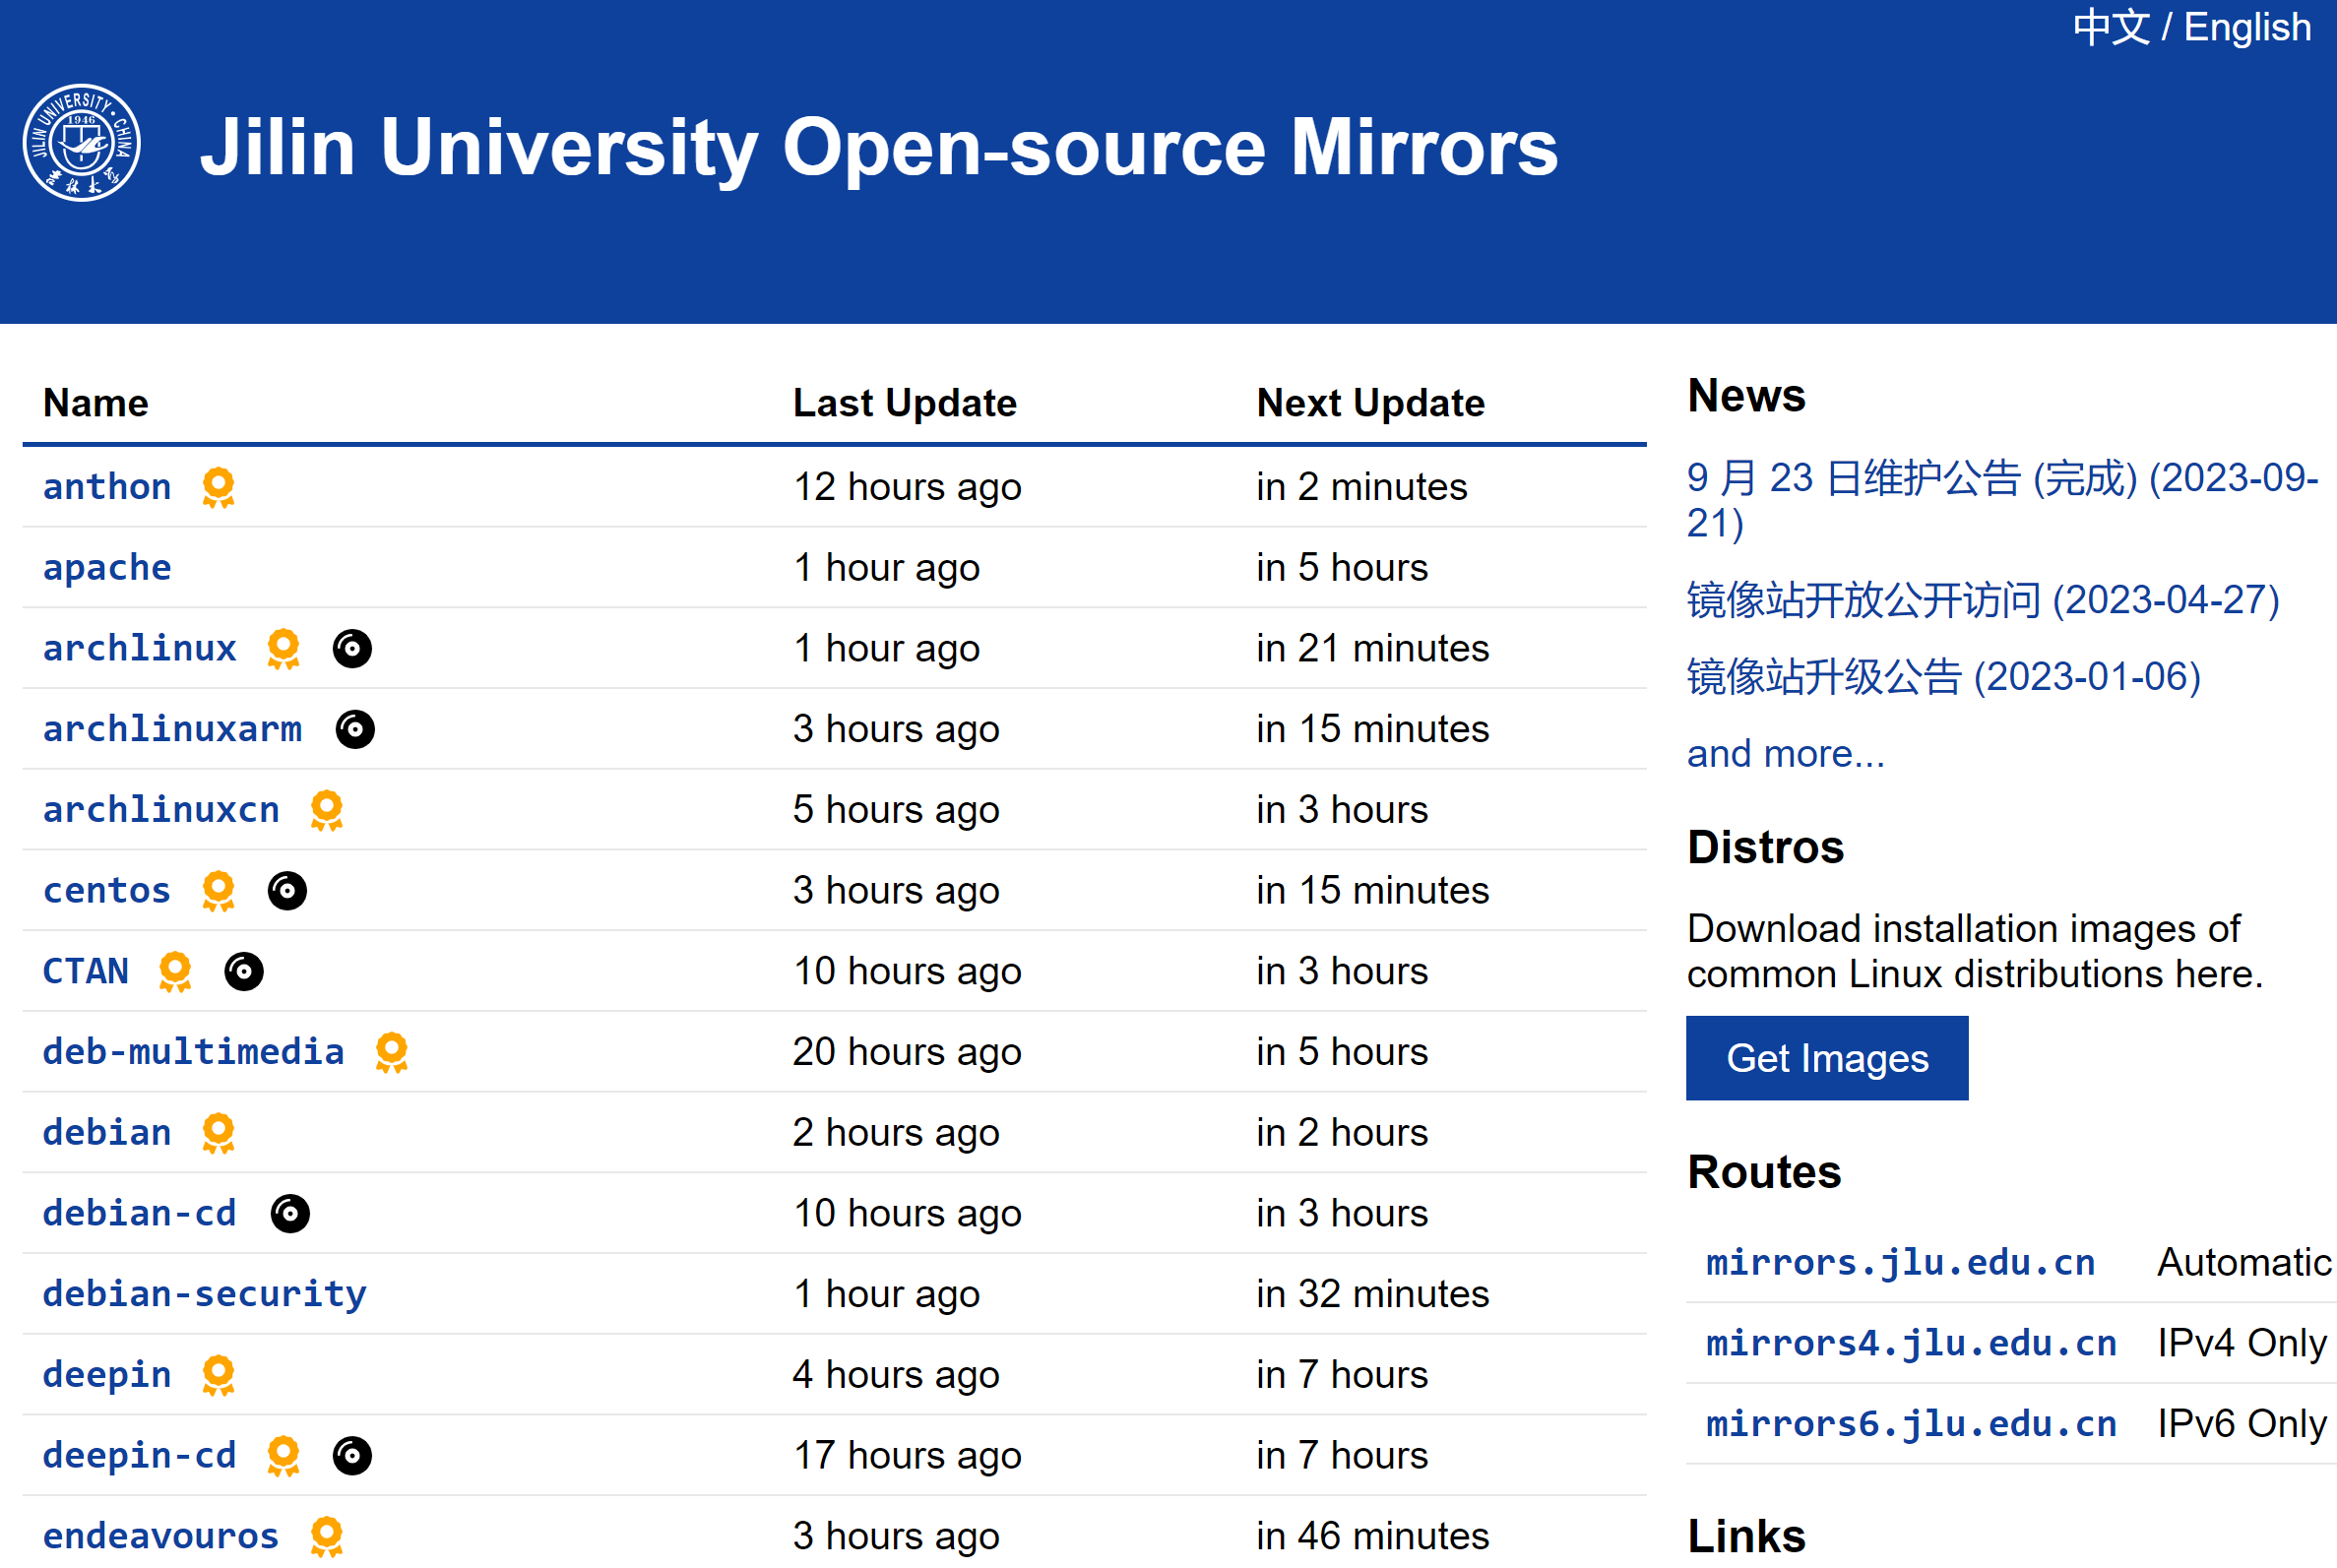
\includegraphics[height=.8\textheight]{pic/mirror.png}
        \caption{https://mirrors.jlu.edu.cn/}
    \end{figure}
\end{frame}

\begin{frame}{mirrors}
    \begin{figure}[c]
        \centering
        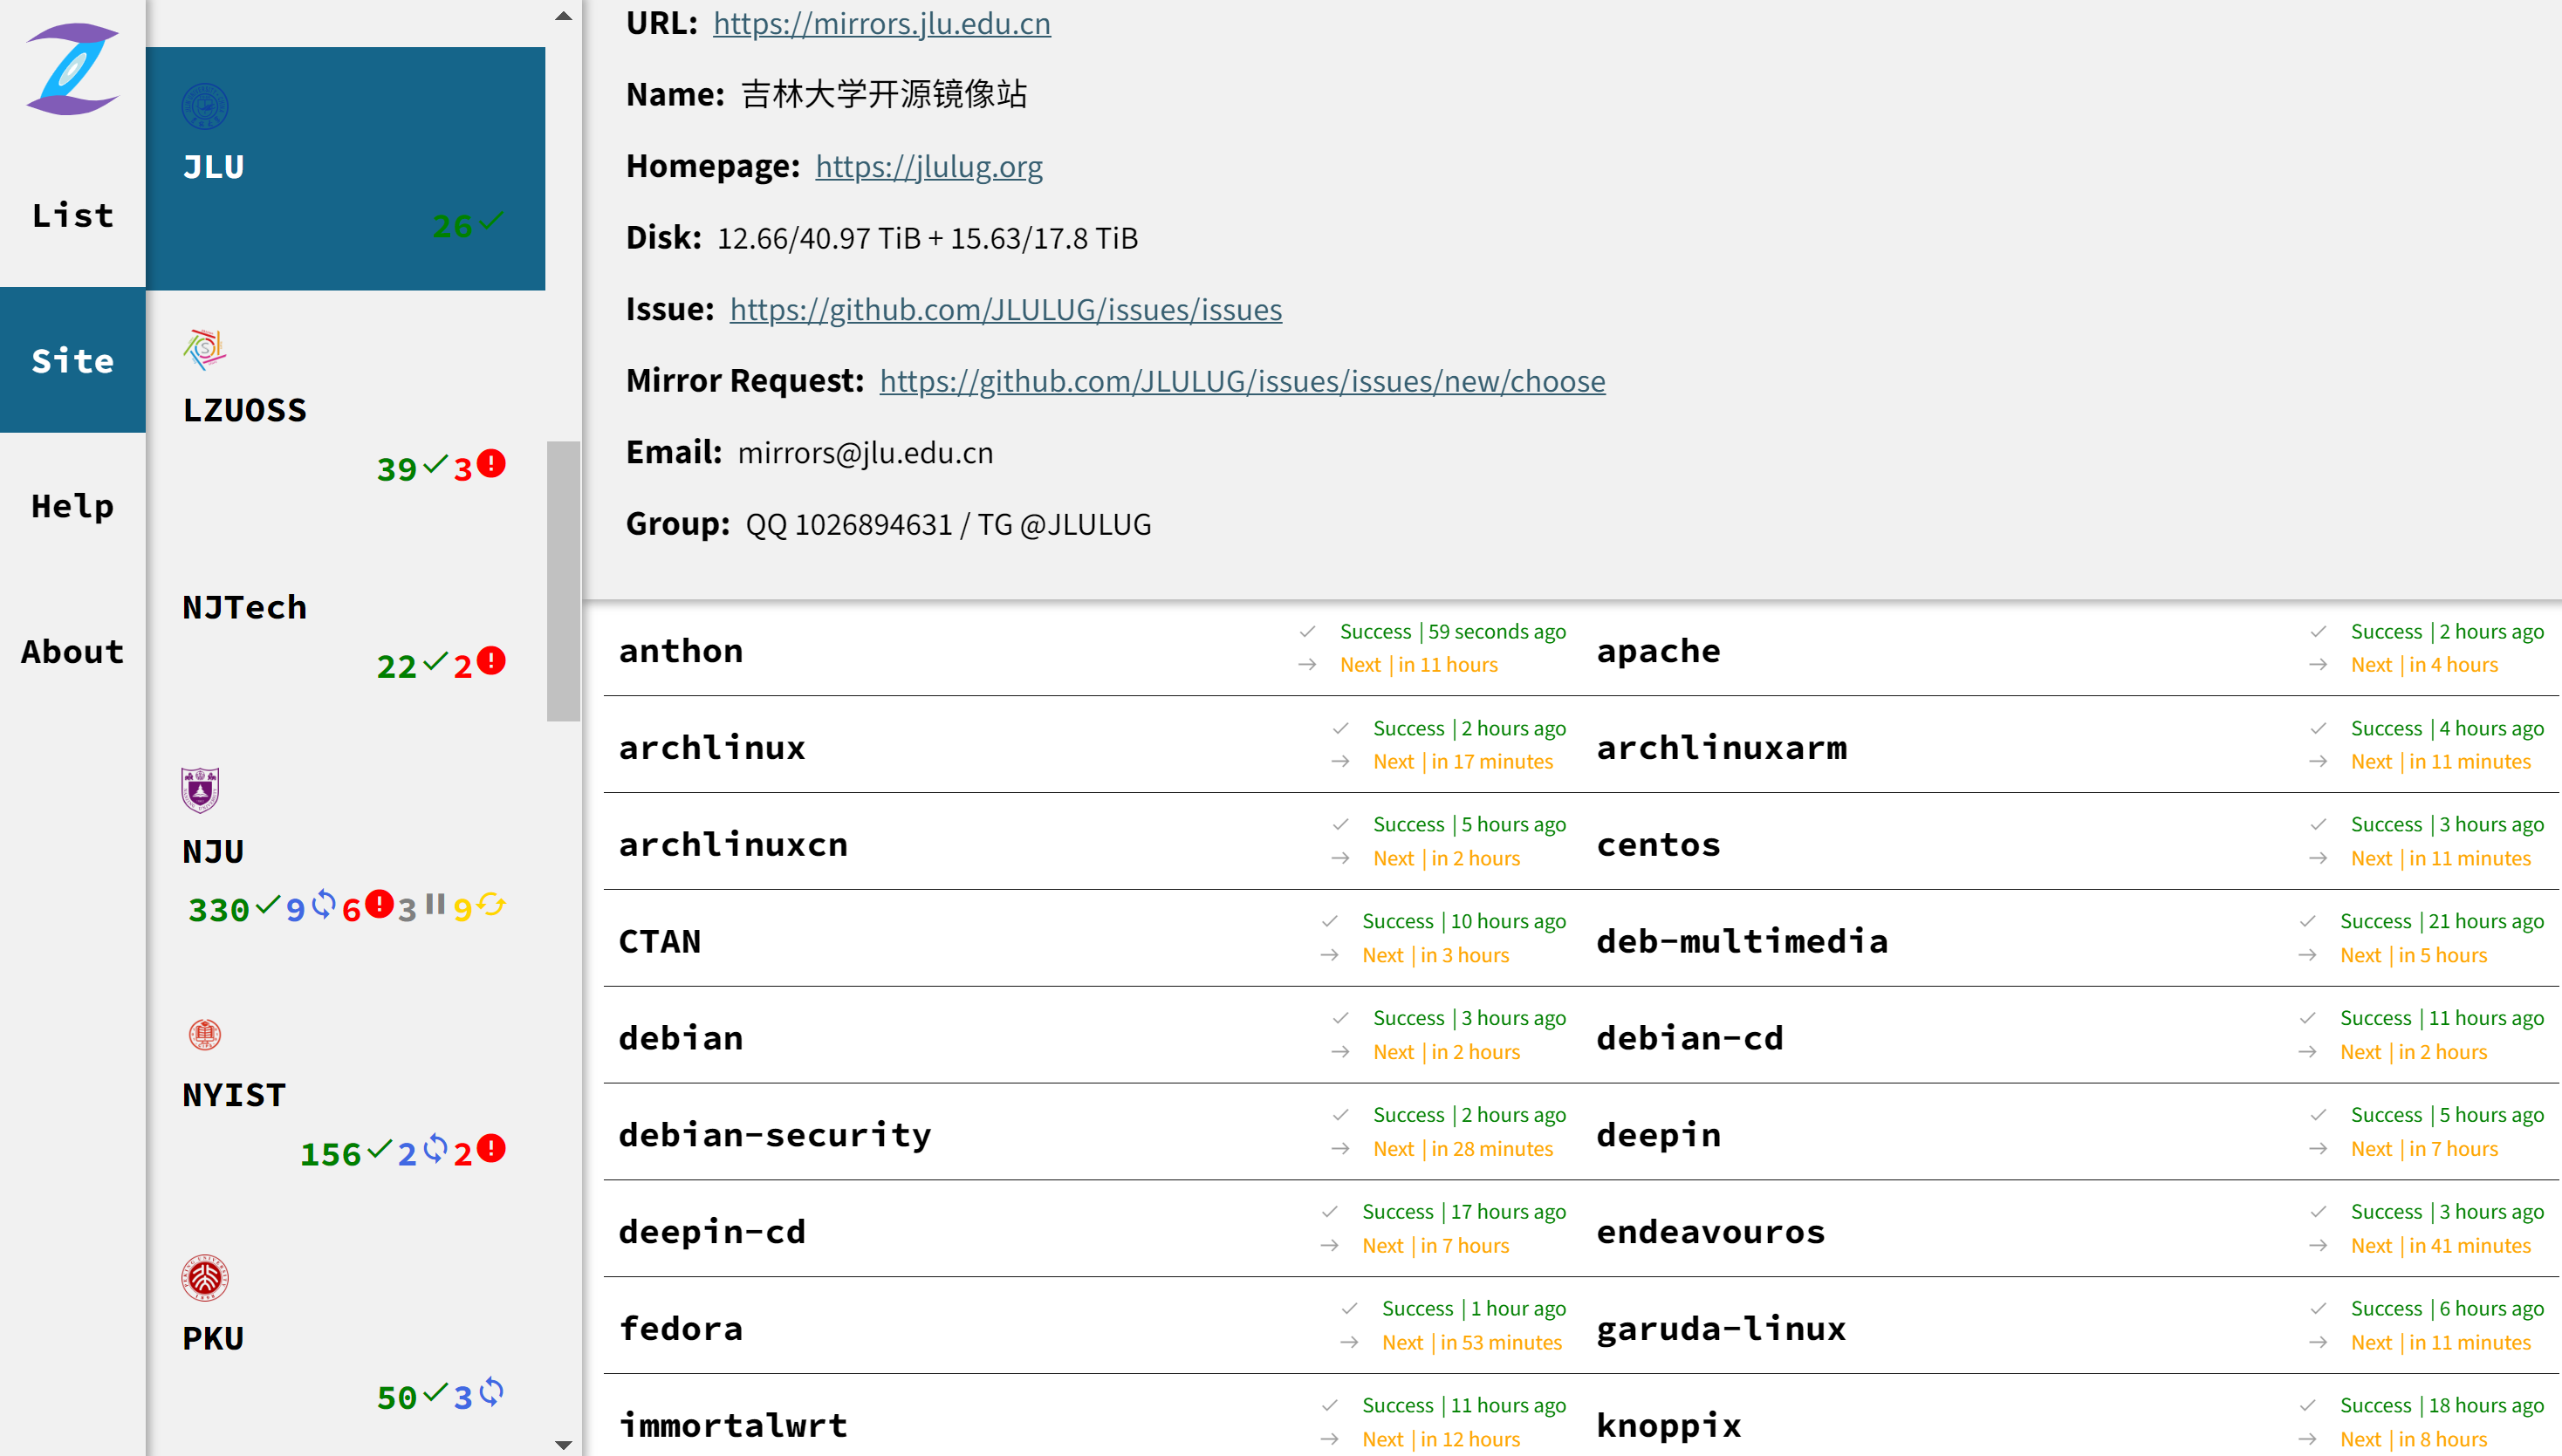
\includegraphics[height=.7\textheight]{pic/mirrorz.png}
        \caption{MirrorZ.org}
    \end{figure}
\end{frame}

\begin{frame}{proxy}
    \begin{itemize}
        \item WebVPN 助手: https://greasyfork.org/scripts/395271
        \item 包管理器使用代理: https://github.com/rosebe/FUCK-GFW
        \item Transparent Proxy
    \end{itemize}
\end{frame}

\begin{frame}{proxy}
    \begin{figure}[c]
        \centering
        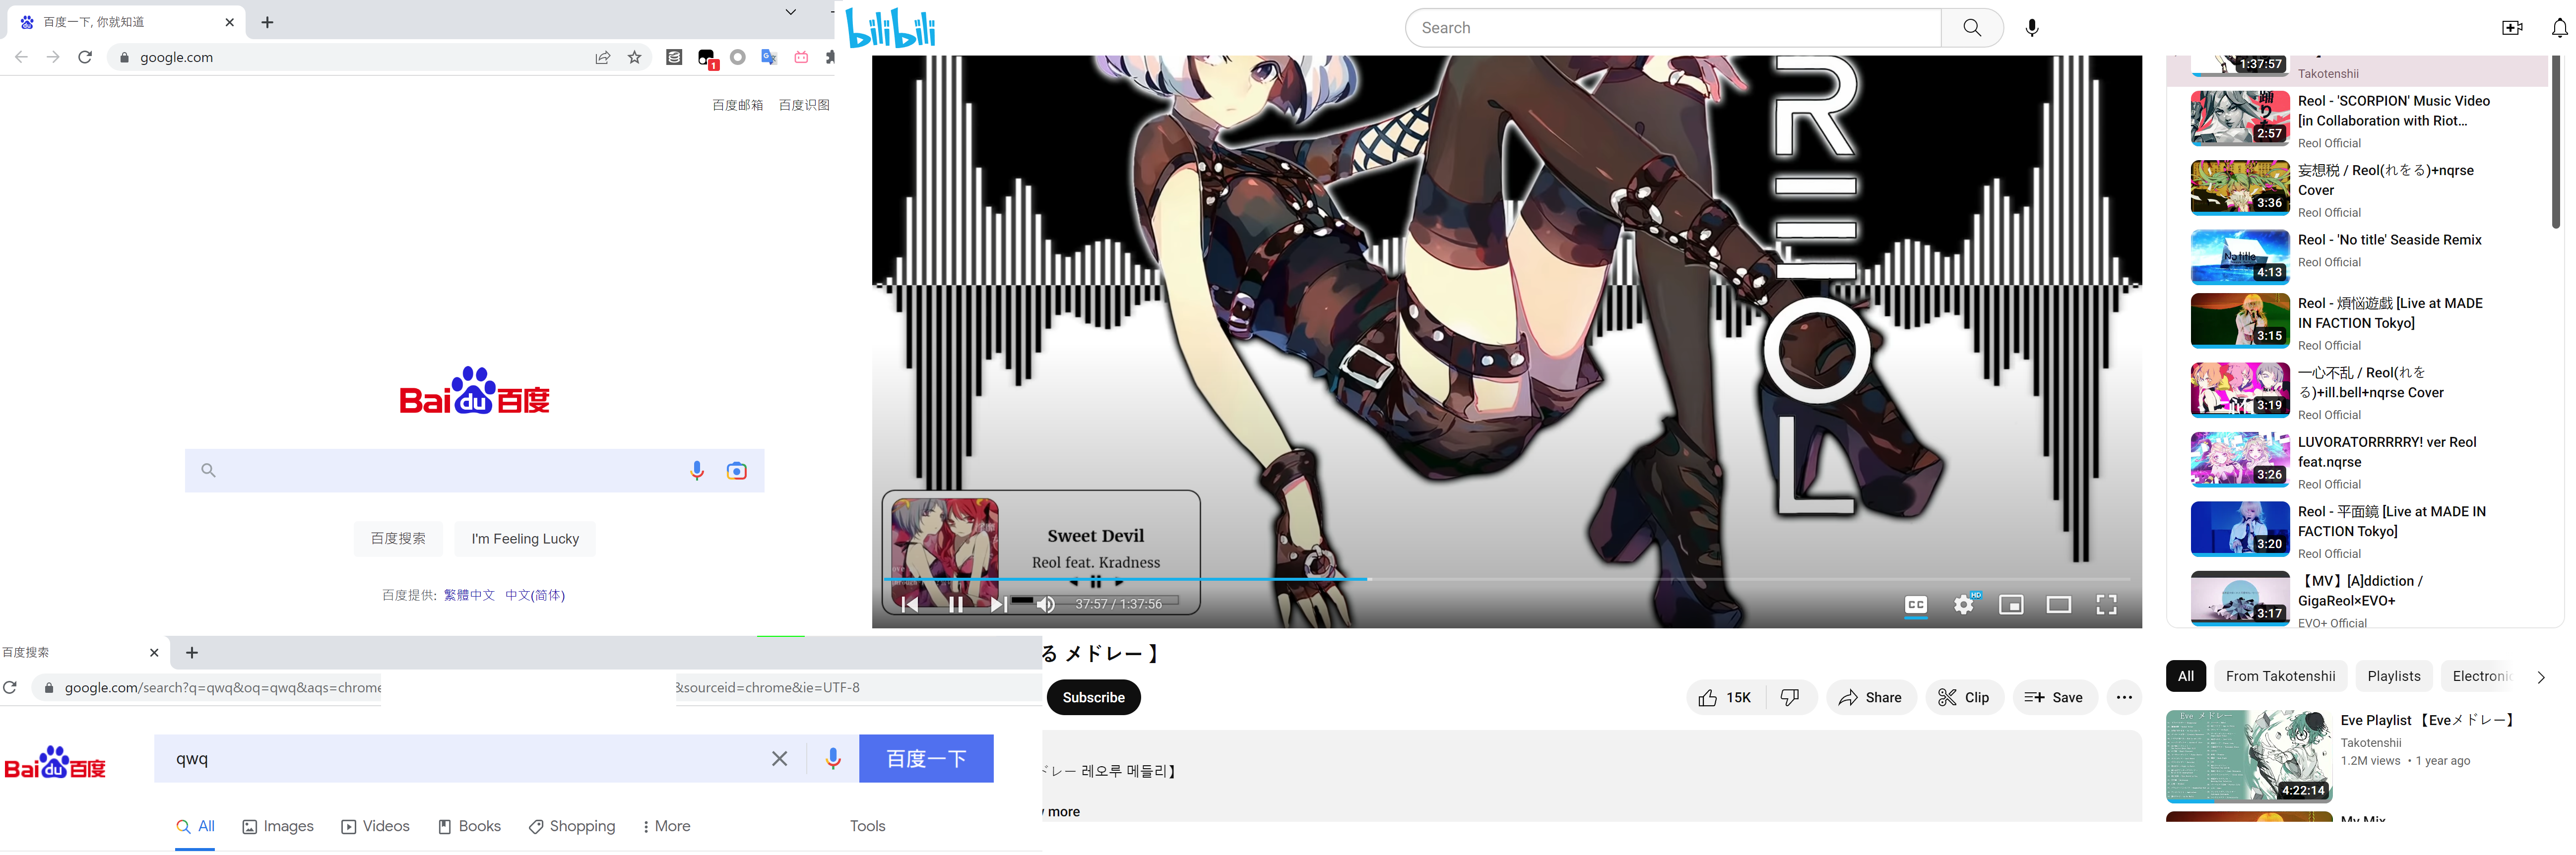
\includegraphics[height=.5\textheight]{pic/gf.png}
        \caption{将国际网站伪装成中国网站}
    \end{figure}
    \begin{itemize}
        \item https://github.com/userElaina/this-is-the-China-website
        \item https://greasyfork.org/scripts/461427
    \end{itemize}
\end{frame}

\begin{frame}{虚拟环境}
    \begin{itemize}
        \item {\tt{py -m venv ENV\_DIR}}
        \item Anaconda / Miniconda
        \item {\tt{conda create -n ENV\_NAME python=x.x}}
        \item Docker
        \item Virtual Machine: WSL, Sandbox, Hyper-V, VirtualBox, VMware, Qemu, PVE, ESXi, ...
    \end{itemize}
\end{frame}

\begin{frame}{虚拟环境 - Windows}
    Control Panel - Programs - Turn Windows features on or off:
    \begin{itemize}
        \item Hyper-V
        \item Windows Hypervisor Platform
        \item Windows Sandbox
        \item Windows Subsystem for Linux
    \end{itemize}
\end{frame}

\section{Linux}

\begin{frame}{Shell}
    Shell is not Terminal!
    \begin{itemize}
        \item bash: Bourne Again Shell, default.
        \item Zsh: Z Shell, https://ohmyz.sh/.
        \item fish: Friendly Interactive Shell, generates by parsing man pages.
    \end{itemize}
\end{frame}

\begin{frame}{Help}
    \begin{itemize}
        \item {\tt ----help}
        \item man
        \item tldr
        \item RTFM, STFW
    \end{itemize}
\end{frame}

\begin{frame}{IDE}
    \begin{itemize}
        \item 编译器: 是将原始语言源代码转换成目标语言计算机程序. gcc, msvc, clang, ...
        \item 编辑器: 文本编辑. Vim, NeoVim, VSCode, ...
        \item 集成开发环境 (IDE): 能编辑, 构建, 测试, 打包的软件. VS, JetBrains, ...
    \end{itemize}
\end{frame}

\begin{frame}{CLI}
    \begin{itemize}
        \item {\tt ls -ahl}: all, human readable, long listing format
        \item diff, 比较文件
        \item cat, bat, 输出与拼接文件
        \item xxd, hexyl, 十六进制输出文件
        \item find, fd, 查找文件
        \item grep, ripgrep, 搜索文件内容
        \item top, htop, btop, "任务管理器"
        \item make, cmake, 自动化
        \item neofetch, 显示系统信息
        \item FFmpeg, 多媒体处理
    \end{itemize}
\end{frame}

\begin{frame}{SSH (SCP)}
    \begin{itemize}
        \tt
        \item ssh-keygen -t ed25519 -C "userelaina@pm.me"
        \item cat \textasciitilde/.ssh/id\_ed25519.pub
        \item ssh-ed25519 AAAAC3NzaC1lZDI1NTE5AAAAIKmmagvzHfnb NiN3mKrLYqCirEm75But9tKxKas5VX4n userelaina@pm.me
        \item vim \textasciitilde/.ssh/id\_ALGORITHM
        \\ \quad \\
        \item ssh -i \textasciitilde/.ssh/id\_ed25519 -p 50022 user@nas.mil
        \item scp -P 50022 -r ./a/ user@192.168.1.2:\textasciitilde/t1/
    \end{itemize}
\end{frame}

\begin{frame}{Git (GitHub)}
    \begin{itemize}
        \item {\tt git clone https://github.com/opencv/opencv.git}
        \item {\tt git clone git@github.com:opencv/opencv.git}
        \item {\tt git clone --recurse-submodules --remote-submodule https://github.com/bad-apple-lab/Bad-Apple.git}
        \\ \quad \\
        \item GitHub - Settings - SSH and GPG keys
        \item {\tt vim \textasciitilde/.ssh/config}
        \item {\tt ssh -T git@github.com}
    \end{itemize}
\end{frame}

\begin{frame}{后台运行}
    \begin{itemize}
        \item \sout{\&}
        \item {\tt nohup CMD > LOG 2>\&1 \&}
        \item screen
        \item Tmux
    \end{itemize}
\end{frame}

\begin{frame}{Distribution}
    \begin{itemize}
        \item Debian and Ubuntu
        \item Arch Linux and Manjaro
        \item RHEL and CentOS
        \item Kali Linux and Black Arch Linux
        \item Deepin
    \end{itemize}
\end{frame}

% \section{硬件}

% \begin{frame}{硬件加速}
%     \begin{itemize}
%     \end{itemize}
% \end{frame}

% \begin{frame}{硬件选购}
%     \begin{itemize}
%     \end{itemize}
% \end{frame}

\section{杂项}

\begin{frame}{Markdown}
    \begin{itemize}
        \item 轻量级文本标记语言 (markup language)
        \item 易读易写, 电子邮件; html; css.
        \item CommonMark, GFM, Pandoc, Typora, ...
        \item VSCode: Markdown Preview Enhanced.
    \end{itemize}
\end{frame}

\begin{frame}{LaTeX}
    \begin{itemize}
        \item 引擎: TeX, pdfTeX, XeTeX, LuaTeX, ...
        \item Why? Template, 专注于内容.
        \item How? LaTeX Workshop, TeXStudio, Overleaf, ...
        \item IEEE
        \item https://github.com/geekifan/jluthesis
        \item https://github.com/jiafeng5513/JLU\_Dissertation
        \item https://github.com/userElaina/Open-JLU
    \end{itemize}
\end{frame}

\begin{frame}{Q \& A}
    \begin{center}
        {\Huge\calligra Thanks!}
    \end{center}
\end{frame}

\end{document}
